%--------------------------------------------------------------------------------------------------
% OBSERVACAO:
% 
% -> Arquivos que você pode editar:
%    - artigo.tex
%    - artigo_bibliografia.bib
%
% -> Arquivo .TeX codificado em UTF8                                                             
% -> Bibliografia em arquivo .bib (arquivo_bibliografia.bib)                                      
% -> Arquivo de imagens em .jpg, .eps ou .pdf
% -> Para compilar o TeX, execute 'compila_TEX.bat' (terminal do windows)
% 
% versão 1.1 - 19/05/2016
% versão 1.0 - 18/08/2015
%--------------------------------------------------------------------------------------------------
\documentclass{classe_cn}                 % Modelo <nao edite o arquivo classe_cn.cls>
\usepackage[brazil]{babel}                % Acentos
\usepackage[utf8]{inputenc}               % Codificação UTF8 (atenção aqui!)
\usepackage{graphicx}                     % Figura
\usepackage{amssymb}                      % Simbolos matematicos
\usepackage{color}                        % Cores
\usepackage{amsfonts}                     % Fontes
\usepackage{amsmath}                      % Fontes
\usepackage[fixlanguage]{babelbib}        % Acentos
\usepackage[normalem]{ulem}               % OK
\usepackage[retainorgcmds]{IEEEtrantools} % Formulas padrão IEEE
\usepackage{omlmathbf}                    % Simbolos Matematicos
\usepackage{epstopdf}                     % Figuras .eps
\usepackage{setspace}                     % Espaçamento flexível
\usepackage{cmap}                         % Mapear caracteres especiais no PDF
\usepackage{textcomp}                     % Funções e outros símbolos matemáticos
\usepackage{verbatim}                     % Pacotes verbatim
\usepackage{wrapfig}
\usepackage{picins}
\startlocaldefs
\endlocaldefs

%--------------------------------------------------------------------------------------------------
% Inicio do Documento
%--------------------------------------------------------------------------------------------------
\begin{document}
\begin{frontmatter}        % Não alterar
\begin{fmbox}              % Não alterar
\dochead{Gerência da Informação} % Não alterar

%--------------------------------------------------------------------------------------------------
% Titulo do seu Trabalho
%   - pequeno bug (nao funciona cedilha)
%   - editar manualmente o cedilha na classe_cn.cls, linha 1015.
%--------------------------------------------------------------------------------------------------
\title{Software Livre para Empresas}

%------------------------------------------------
% Informações sobre o autor #1
% - Antunes Dantas da Silva
%------------------------------------------------
\author[
  addressref = {aff1},                 % Identifica o autor #1
  email      = {antunes.dantas@ccc.ufcg.edu.br} % email para contato
]
{
  \inits{ADdS}      % Letras iniciais do autor #1
  \fnm{Antunes Dantas}  % Nome do autor #1 (first and middle name)
  \snm{da Silva}   % Ultimo nome do autor #1 (last name)
}
%------------------------------------------------
% Informações sobre o autor #2
% - Gabriel Silva Vinha
%------------------------------------------------
\author[
  addressref = {aff1},                      % Identifica o autor
  email      = {gabriel.vinha@ccc.ufcg.edu.br} % email para contato
]
{
  \inits{GSV}       % Letras iniciais do autor #2
  \fnm{Gabriel Silva}  % Nome do autor #2 (first and middle name)
  \snm{Vinha}    % Ultimo nome do autor #2 (last name)
}
%------------------------------------------------
% Informações sobre o autor #3
% - Italo M. de L. Poroca
%------------------------------------------------
\author[
  addressref = {aff1},                       % Identifica o autor
  email      = {italo.poroca@ccc.ufcg.edu.br} % email para contato
]
{
  \inits{IMdLP}      % Letras iniciais do autor #3
  \fnm{Italo M. de Lima} % Nome do autor #3 (first and middle name)
  \snm{Poroca}    % Ultimo nome do autor #3 (last name)
}
%------------------------------------------------
% Informações sobre o autor #4
% - Valter V. M. de Lucena
%------------------------------------------------
\author[
  addressref = {aff1},                 % Identifica o autor
  email      = {valter.lucena@ccc.ufcg.edu.br} % email para contato
]
{
  \inits{VVMdL}     % Letras iniciais do autor #4
  \fnm{Valter V. M.} % Nome do autor #4 (first and middle name)
  \snm{de Lucena}     % Ultimo nome do autor #4 (last name)
}

%------------------------------------------------
% Endereço dos autores
%------------------------------------------------
\address[id=aff1]{
  \orgname{Universidade Federal de Campina Grande,
           Centro de Engenharia Elétrica e Informática,
           Departamento de Sistemas e Computação},
  \street{Rua Aprígio Veloso, 882, Bairro Universitário},
  \postcode{58429-140},
  \city{Campina Grande},
  \cny{Brasil.}
}

\end{fmbox}

%--------------------------------------------------------------------------------------------------
% Resumo do Trabalho
%--------------------------------------------------------------------------------------------------
\begin{abstractbox}
	
\begin{abstract} 
Escrever no máximo $150$ palavras no resumo do trabalho. Exemplo: The objective of this work is to determine if people are interacting in TV video by detecting whether they are looking at each other or not.We determine both the temporal period of the interaction and also spatially localize the relevant people. We make the following four contributions: (\textit{i}) head detection with implicit coarse pose information (front, profile, back); (\textit{ii}) continuous head pose estimation in unconstrained scenarios (TV video) using Gaussian process regression; (\textit{iii}) propose and evaluate several methods for assessing whether and when pairs of people are looking at each other in a video shot; and (\textit{iv}) introduce new ground truth annotation for this task, extending the TV human interactions dataset. The performance of the methods is evaluated on this dataset, which consists of $300$ video clips extracted from TV shows. Despite the variety and difficulty of this video material, our best method obtains an average precision of $87.6\%$ in a fully automatic manner.
\end{abstract}

%--------------------------------------------------------------------------------------------------
% Palavras-chaves: Entre 3 e 6 palavras chaves
%--------------------------------------------------------------------------------------------------
\begin{keyword}
  \kwd{Escreva}
  \kwd{algumas}
  \kwd{palavras-chaves}
  \kwd{aqui!}
\end{keyword}

\end{abstractbox} % Não alterar
\end{frontmatter} % Não alterar

%--------------------------------------------------------------------------------------------------
% Escreva o seu artigo!
%--------------------------------------------------------------------------------------------------

%------------------------------------------------
% Seção 1
%------------------------------------------------
\section{Introdução}

Escreva introdução e motivação do seu trabalho. Tente convencer o leitor da importância da sua pesquisa. Exemplo: If you read any book on film editing or listen to a director's commentary on a DVD, then what emerges again and again is the importance of eyelines. Standard cinematography practice is to first establish which characters are looking at each other using a medium or wide shot, and then edit subsequent close-up shots so that the eyelines match the point of view of the characters. This is the basis of the well known $180^{o}$ rule in editing.

The objective of this paper is to determine whether eyelines match between characters within a shot—and hence understand which of the characters are interacting~\cite{Pressman:2007}. The importance of the eyeline is illustrated by the three examples of Figure~\ref{tag_figura_01} - one giving rise to arguably the most famous quote from Casablanca, and another being the essence of the humour at that point in an episode of Fawlty Towers. Our target application is this type of edited TV video and films. It is very challenging material as there is a wide range of human actors, camera viewpoints and ever present background clutter. The thirty Brodatz textures u asl sklsksj slk slk dsed are shown in Figure~\ref{tag_figura_01}.

begin
\begin{figure}[h!]
  \begin{center}
    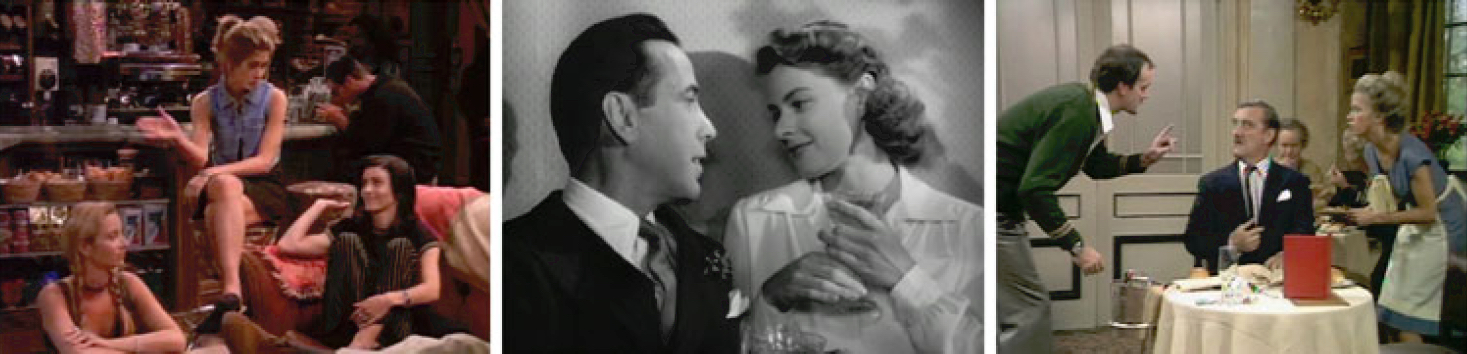
\includegraphics[width=1.0 \textwidth]{figura01.jpg}
    \caption{Exemplo de Figura 01.} 
    \label{tag_figura_01}
  \end{center}
\end{figure}

Gray level co-occurrence matrix (GLCM)~\cite{Ferris:2003} describes the relative frequencies with which two pixels separated by a distance $d$ under a specified angle occur on the image. Then, the GLCM matrices are pre-processed in order to obtain input data for the clustering or classification modules. In the Clustering module the SOM neural network organises and extracts prototypes from the processed matrices, which ends the learning stage. The classification module receives a pre-processed query image and compares it with the prototypes (representations of clusters) obtained in the clustering module. The final result is a list of images belonging to a few number of clusters considered to be the nearest to the user's query. Figure~\ref{tag_figura_02} shows these building blocks.

\begin{figure}[h!]
  \begin{center}
    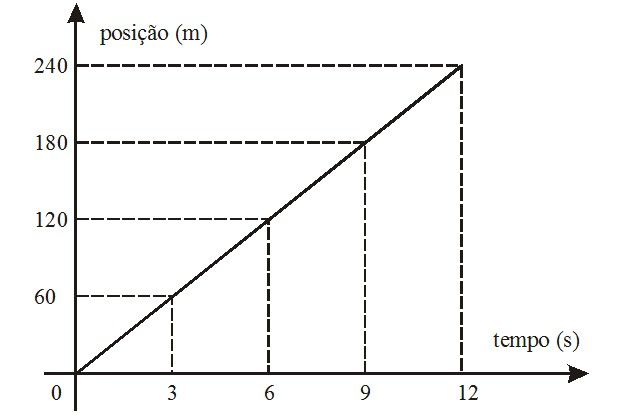
\includegraphics[width=1.0 \textwidth]{figura02.jpg}
    \caption{Exemplo de Figura 02.} 
    \label{tag_figura_02}
  \end{center}
\end{figure}

%------------------------------------------------
% Seção 2
%------------------------------------------------
\section{Motivação}

If we assume that sensitive cells follow a deterministic decay $Z_0(t) = xe^{\lambda_0 t}$ and approximate their extinction time as $T_x \approx \frac{1}{\lambda_0} \log x$, then we can heuristically estimate the expected value as:

\begin{eqnarray}
\label{eqexpmuts}
  E [Z_1(vT_x)] &=& \frac{\mu}{r}\log x \int_0^{1} x^{1-u} du \\
  E [Z_1(vT_x)] &=& \frac{\mu}{r}x^{1-{\lambda_1}/{\lambda_0}v}\log  \\
  1 &=& 10
\end{eqnarray}

\begin{equation}
  E [Z_1(vT_x)] = \frac{\mu}{r}\log x \int_0^{1} x^{1-u} du \\
  E [Z_1(vT_x)] = \frac{\mu}{r}x^{1-{\lambda_1}/{\lambda_0}v}\log 
\end{equation}

Thus we observe that this expected value is finite for all $v>0$ (also see \cite{Rosenfeld:1970}).

%------------------------------------------------
% Sub-seção
%------------------------------------------------
\subsection{Exemplo de Sub-Seção}

In this section we examine the growth rate of the mean of $Z_0$, $Z_1$ and $Z_2$. In addition, we examine a common modeling assumption and note the importance of considering the tails of the extinction time $T_x$ in studies of escape dynamics. We will first consider the expected resistant population at $vT_x$ for some $v>0$, (and temporarily assume $\alpha=0$).

\begin{eqnarray}
E [Z_1(vT_x)]= \mu T_x \int_{0}^{\inf} \lambda_1T_x(v-u)du
\end{eqnarray}

If we assume that sensitive cells follow a deterministic decay $Z_0(t)=xe^{\lambda_0 t}$ and approximate their extinction time as $T_x\approx-\frac{1}{\lambda_0}\log x$, then we can heuristically estimate the expected value as.

%------------------------------------------------
% Exemplo de Tabela
%------------------------------------------------
\section{Software Livre}

Por \textit{Software} Livre entende-se aquele que respeita a liberdade e o censo de comunidade do usuário. Isto é, todo o \textit{software} que pode ser usado, copiado, estudado, modificado e redistribuído sem restrições.

Durante a década de 60, quando os computadores eram mais utilizados em empresas e instituições governamentais, não havia a ideia de \textit{software} e \textit{hardware} como algo separado, do ponto de vista comercial. Em geral, o \textit{software} era entregue junto com o código-fonte, ou apenas este último era entregue. Devido a isso, grupos e comunidades de usuários que trocavam informações e compartilhavam código eram comuns. A partir daí, pode-se afirmar que o \textit{software} era livre, em suas origens.

Ainda nessa mesma década, sistemas operacionais e compiladores de linguagens de programação começaram a evoluir, aumentando drasticamente seus custos. Assim, uma indústria pequena e crescente começava a surgir, competindo diretamente com os \textit{softwares} entregues juntos ao \textit{hardware}. Em 1970, a IBM, líder do mercado de computadores da época, anunciou que a partir daquele ano passaria a vender parte de seus programas separada das máquinas. Com isso, a indústria de \textit{software} tomou um rumo em que restrições de acesso e de compartilhamento de código entre desenvolvedores ficaram cada vez mais comuns.

Em 1978, Donald Knuth professor da Universidade de Stanford, começou a trabalhar no TeX, sistema de tipografia popular até hoje no meio acadêmico, que foi distribuído com a ideia de que qualquer um pudesse usá-lo sem restrições (seu código-fonte estava em uma seção do volume 2 do seu livro \textit{The Art of Computer Programing}). A partir daí, a ideia base do \textit{software} livre como conhecido hoje começou a surgir.

Em 1983, Richard Stallman, funcionário do MIT, teve uma experiência negativa com \textit{software} comercial, e deu origem ao Projeto GNU. Durante o período que estava no MIT, identificou uma falha no \textit{software} de uma impressora. Ao tentar corrigí-lo, a empresa se negou disponibilizar o código-fonte. Isso o motivou a criar um mecanismo legal de garantia para que todos pudessem desfrutar dos direitos de copiar, redistribuir e modificar \textit{Software}, dando origem à licença GPL. Para institucionalizar o Projeto GNU, Stallman fundou a Free Software Foundation. Nasce assim o Movimento do \textit{Software} Livre.

Em julho de 1991, Linus Torvalds, estudante da Universidade de Helsinki - Finlândia, divulgou nota com menções sobre seu projeto de construir um núcleo operacional livre, similar ao Minix, e obteve ajuda de vários desenvolvedores ao redor do mundo. Em setembro do mesmo ano, Linus lançou a versão oficial do que hoje é o Linux. Centenas de desenvolvedores se juntaram ao projeto para integrar todo o sistema GNU (compilador, editor de textos, shell, etc) em torno do núcleo do Linux. Nasce então, sob a licença GPL, o sistema operacional GNU/Linux.

Após isso, o movimento do \textit{software} livre vem crescendo com grandes projetos, tais como todas as distribuições do Linux, o OpenStack, o Eclipse, e empresas, como a RedHat, Canonical, Free Software Foundation -- como já citada --, entre outras.

Algo a ser esclarecido é que \textit{software} livre é diferente de \textit{software} em domínio público e de \textit{software} gratuito. Em domínio público, significa que seu autor abriu mão dos seus direitos autorais. E quanto a ser gratuito, pode citar os serviços de \textit{cloud-computing} da RedHat, e a distribuição Suse Linux, com foco empresarial, que não são gratuitos.

Entram então alguns conceitos importantes a respeito de \textit{software} livre, tais como \textit{software} como um produto (SaaP), \textit{software} como um serviço (SaaS) e os componentes da procução de \textit{software}.


\subsection{Software as a Product}

\textit{Software as a Product}//citação aqui?? -- ou \textit{Software} como um Produto, em tradução livre --

\subsection{Software as a Service}

olar

\subsection{Componentes da Produção de Software}

acesso ao software

\section{Licenças de Publicação}

tarara

\section{Software Livre Para Empresas}


\subsection{estatisticas de mercado para saap}
oi


\subsection{Software as a service}

aqui vc faz

\subsection{core}

\section{Tendências}

olar


%--------------------------------------------------------------------------------------------------
%--------------------------------------------------------------------------------------------------
% Define o arquivo BIB (bibliografia)
%--------------------------------------------------------------------------------------------------
%--------------------------------------------------------------------------------------------------
\bibliographystyle{bmc-mathphys}   % NAO EDITAR!
\bibliography{artigo_bibliografia} % NAO EDITAR! - Bibliography file (usually '*.bib' )

\vspace{1.0cm}
\parpic{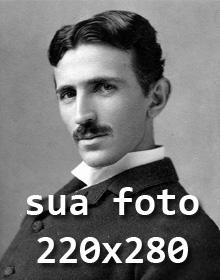
\includegraphics[width=1.5in,clip,keepaspectratio]{tesla.jpg}}
\noindent {\bf Fulano de Tal} was born in India. She received the B.S. 
degree in computer science from Kurukshetra University, Kurukshetra, 
India and the M.Phil. and Ph.D. degrees from the University of Exeter, 
Exeter, UK in 1999, 2001 and 2004, respectively. Her Ph.D. was in the 
area of machine learning for image analysis in aviation security. Her 
main research interests include image processing, natural scene analysis,
video analysis, and neural networks. She has published more than 30 papers
in the area of machine learning for image analysis in peer reviewed 
journals and conferences. Currently she is a Senior Research Fellow at
Loughborough University leading the project on imaging for road transport
applications.

\parpic{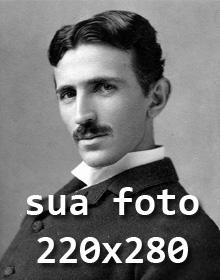
\includegraphics[width=1.5in,clip,keepaspectratio]{tesla.jpg}}
\noindent {\bf Fulano de Tal} was born in India. She received the B.S. 
degree in computer science from Kurukshetra University, Kurukshetra, 
India and the M.Phil. and Ph.D. degrees from the University of Exeter, 
Exeter, UK in 1999, 2001 and 2004, respectively. Her Ph.D. was in the 
area of machine learning for image analysis in aviation security. Her 
main research interests include image processing, natural scene analysis,
video analysis, and neural networks. She has published more than 30 papers
in the area of machine learning for image analysis in peer reviewed 
journals and conferences. Currently she is a Senior Research Fellow at
Loughborough University leading the project on imaging for road transport
applications.   


%\end{tabular}
%\end{table}

%--------------------------------------------------------------------------------------------------
% FIM DO ARTIGO
%--------------------------------------------------------------------------------------------------
\end{document}
